\documentclass[aps,rmp,preprint,superscriptaddress,10pt,twocolumn]{revtex4-1}
\usepackage[utf8x]{inputenc}
\usepackage{amsmath,amsthm,amsfonts,amssymb,amscd}
\usepackage{graphicx}
\usepackage{wrapfig}
\usepackage{enumerate}
\usepackage{color}
\usepackage[final]{hyperref}
\usepackage{fontspec}
%\usepackage{natbib}
%\bibliographystyle{plainnat}


\setmainfont{Times New Roman}

%\setlength{\parindent}{20pt}
\def\thesubsectiondis{\unskip\arabic{subsection}}
 
\begin{document}

\title{Structural diversity around mobile beta-lactamase genes}
\author{Liam P. Shaw}
\email{liam.shaw@biology.ox.ac.uk}
\affiliation{Department of Biology, University of Oxford, Oxford, UK\looseness=-5}
\affiliation{Department of Biosciences, University of Durham, Durham, UK\looseness=-5}
\author{Richard A. Neher}
\affiliation{Biozentrum, University of Basel, Basel, Switzerland\looseness=-5}

\begin{abstract}
Since the introduction of penicillin, the first beta-lactam antibiotic, surveillance of clinical bacteria has tracked the increasing prevalence of novel beta-lactamases. These key antibiotic resistance genes typically spread worldwide within decades on mobile genetic elements (MGEs), both within and between species. On these timescales, MGEs evolve not by point mutation but through larger-scale structural rearrangements. The structural diversity of the flanking regions around each gene makes attempts to understand their spread challenging. Previous studies have analysed individual genes using bespoke methods, making it difficult to compare between them to understand the general processes involved in their evolution. Here, we use a pangenome analysis tool (PanGraph) to apply a consistent approach to the genetic contexts of clinically relevant beta-lactamases from twelve enzyme families. Our findings give insight into the general rules that apply to the horizontal spread of new beneficial genes through bacterial populations.    
\end{abstract}


\maketitle

\section{Introduction}

\noindent Beta-lactam antibiotics are key to modern medicine. They account for 65\% of prescriptions for injectable antibiotics in the United States \cite{Bush2016}. Although beta-lactam antibiotics have diverse structures, they share a common component in the `beta-lactam ring', first seen in the structure of penicillin \cite{Chain1946}. The beta-lactam ring is what allows a beta-lactam antibiotic to bind to certain proteins and as a result inhibit the biosynthesis of the cell wall \cite{Park1957}. Once these proteins are bound, the bacterium cannot form the cross-links between peptides that produce peptidoglycan, prompting a `futile cycle' of cell wall synthesis and degradation that induces cell death \cite{Cho2014}.\par

Penicillin was the first beta-lactam to be mass-manufactured, but it was followed by many others. Today, the WHO Anatomical Therapeutic Chemical (ATC) classification of antibacterials for systemic use includes 93 different beta-lactam molecules: 37 penicillins, 47 cephalosporins, 2 monobactams, and 7 carbapenems \cite{WHO_ATC}. Resistance to beta-lactam antibiotics can be provided by beta-lactamases. Any enzyme which hydrolyses the beta-lactam ring, breaking it apart and removing its antibacterial activity, is classed as a beta-lactamase. The beta-lactamases are a diverse class of enzymes classified into broad enzyme families, with different hydrolytic activities against different beta-lactams \cite{Bush2016}.\par 

Beta-lactams are naturally occurring molecules, and similarly the beta-lactamases are ancient enzymes. The first bacterial enzyme able to `destroy' penicillin was reported in 1940 {--} the year before penicillin was used to treat patients \cite{Abraham1940}. As well as phylogenetic estimates that date the origin of particular enzyme families to billions of years before the present \cite{Barlow2002, Hall2004}, physical evidence confirms that beta-lactamases pre-date the antibiotic era. Beta-lactamases have been discovered in samples from early 13th century Anatolia \cite{Devault2017}, 30,000-year-old permafrost in the Yukon \cite{Dcosta2011}, and a cave system isolated for 4 million years \cite{Bhullar2012}. 

Their natural origins notwithstanding, the clinical use of beta-lactams exerts a strong selective pressure for bacteria to carry beta-lactamases. This effect was visible almost immediately after the widespread introduction of penicillin in the 1940s. At one London hospital, the proportion of penicillin-resistant \textit{Staphylococcus aureus} increased from 14\% in 1946 to 59\% in 1948 \cite{Barber1949}. Today, beta-lactamases are most problematic in Gram-negative species\cite{Bush2020}, with WHO designating them priority pathogens for the development of new antibiotics \cite{WHO2017}. Beta-lactamases are a global health concern, with recent estimates suggesting much higher prevalences in the Global South \cite{Global2022}. A particular concern are extended-spectrum beta-lactamases (EBSLs) which confer resistance to a range of beta-lactams \cite{Livermore2008}. Where good data is available, it suggests that the prevalence of ESBLs is increasing in clinical bacteria. For example, one US study of urinary \textit{E. coli} isolates reported a steady increase from 4.1\% in 2011 to 7.3\% in 2019 \cite{Kaye2021}. \par

One of the reasons for the rapid spread and diversification of beta-lactamases is their horizontal transfer. Many clinically important beta-lactamases are carried on mobile genetic elements (MGEs) such as plasmids or transposable elements. The evolution of these novel plasmid-mediated beta-lactamases has developed both from mutations in existing plasmid-mediated beta-lactamases {--} such as the G238S mutation in SHV-1 to produce SHV-2 which could hydrolyze expanded-spectrum cephalosporins \cite{Bradford2001} {--} and from the mobilization of previously chromosomal beta-lactamases \cite{Bush2020}. \par

Analysing a mobile gene across different genomic backgrounds is challenging, because there is typically vast structural diversity surrounding the gene. The many rearrangement events in the flanking regions mean that traditional alignment approaches are inappropriate. As an example, the metallo-beta-lactamase NDM-1 was first reported in 2008 \cite{Yong2009}. A retrospective search has found samples only as far back as 2005 \cite{Jones2014}. By the 2010s NDM-1 had been seen worldwide; as of this year, it is present in NCBI whole-genome sequencing data from seventeen bacterial genera \cite{CARD2023} and . Such a rapid global spread via horizontal genetic transfer presents a challenge for genomic analysis. Examining the flanking regions surrounding NDM-1 shows large structural diversity, particularly upstream, but with downstream patterns that suggest that NDM-1 was first mobilized by a Tn\textit{125} transposon \cite{Toleman2012, Acman2022}. However, since most analyses focus only on a single gene at a time, it is unclear if there are general rules that govern the mobilisation of beta-lactamases and the subsequent degradation of their ancestral elements, or whether each gene represents a special case. \par 

Recent graph-based approaches to analysing pangenomes such as PanGraph \cite{Noll2022} can accommodate highly dynamic accessory genomes. They provide a general methodology to quantify structural diversity around different beta-lactamases. Here, we apply PanGraph to a dataset of complete chromosome and plasmids carrying beta-lactamases, aiming to offer a quantitative picture of the structural diversity surrounding them. The rapid spread of different beta-lactamases is a chance to witness the dynamics that govern the arrival and establishment of a beneficial gene within a species pangenome. 


\begin{table*}[ht]
\begin{small}
\begin{tabular}{p{0.25\linewidth}p{0.25\linewidth}p{0.25\linewidth}}
\textbf{Enzyme family} & \textbf{Functional group} & \textbf{Members}                  \\
CMY            & 1, 1e                        & CMY-1 to CMY-50                         \\
TEM         & 2b                           & TEM-1, TEM-2, TEM-13                 \\
               & 2be                          & TEM-3, TEM-10, TEM-26                    \\
               & 2br                          & TEM-30 (IRT-2), TEM-31 (IRT-1), TEM-163 \\
               & 2ber                         & TEM-50 (CMT-1), TEM-158 (CMT-9)         \\
SHV            & 2b                           & SHV-1, SHV-11, SHV-89                   \\
               & 2be                          & SHV-2, SHV-3, SHV-115                   \\
               & 2br                          & SHV-10, SHV-72                          \\
CTX-M          & 2be                          & CTX-M-1, CTX-M-44 (Toho-1) to CTX-M-92  \\
PER            & 2be                          & PER-1 to PER-5                          \\
VEB            & 2be                          & VEB-1 to VEB-7                          \\
GES            & 2f                           & GES-2 to GES-7 (IBC-1) to GES-15        \\
KPC            & 2f                           & KPC-2 to KPC-13                         \\
OXA            & 2d                           & OXA-1, OXA-2, OXA-10                    \\
               & 2de                          & OXA-11, OXA-14, OXA-15                  \\
               & 2df                          & OXA-23 (ARI-1), OXA-51, OXA-58, OXA-48         \\
IMP            & 3a                           & IMP-1 to IMP-26                         \\
VIM            & 3a                           & VIM-1 to VIM-23                         \\
NDM             & 3a                            & NDM-1
\end{tabular}
\end{small}
\caption{Major families of $\beta$-lactamases of clinical importance selected for analysis in this study. Adapted from Table 2 of \textcite{Bush2010}.}
\label{table:families}
\end{table*}
% TODO: adapt further to connect to the clusters that I actually look at here. Probably don't need the functional group assignments? Need to decide if ordering alphabetically or via functional group.



\section{Methods}

\begin{figure}
    \centering
    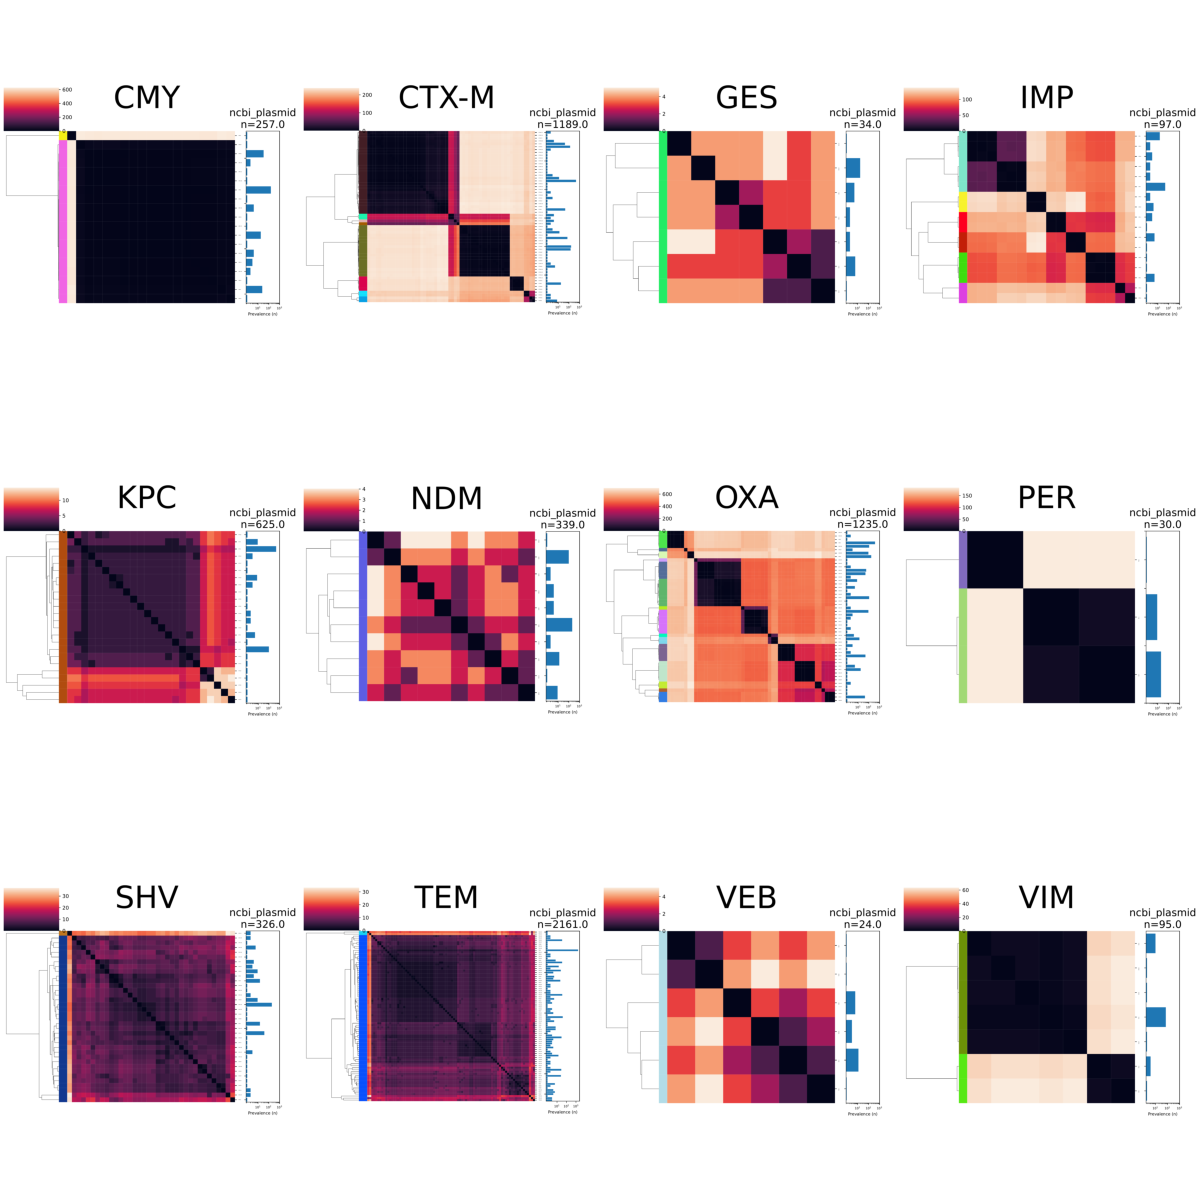
\includegraphics[width=\linewidth]{figs/COMBINED_ncbi_plasmid.pdf}
    \caption{Sequence diversity within named variants in twelve beta-lactamase enzyme families. While most families (e.g. NDM) represent very limited sequence variation, the OXA family encompasses highly diverse non-homologous enzymes. The CTX-M enzymes contain the CTX-M-1 group (inc. CTX-M-55) and CTX-M-9 group as well as intermediate `hybrids' such as CTX-M-123, which was likely formed by homologous recombination between the two groups \cite{He2013}.}
    \label{fig:family-alignments-plasmid}
\end{figure}
% TODO: replace with NJ trees of the actual variation within the focal gene clusters?

\paragraph*{Beta-lactamase families.} Based on a review of the literature and the classification of clinically important beta-lactamase families \cite{Bush2010} we chose twelve clinically important beta-lactamase enzyme families: CMY, TEM, SHV, CTX-M, PER, VEB, GES, KPC, OXA, IMP, VIM, NDM.\footnote{We investigated IND and SME but excluded them due to very little available genomic data.} The sequence diversity of named variants within these enzyme families (Fig. \ref{fig:family-alignments-plasmid}) showed that most include few SNPs and can be treated as recent diversification of a single gene. However, some e.g. OXA include multiple non-homologous enzymes. 

\paragraph*{Dataset.} We used prevalence data from the Comprehensive Antibiotic Resistance Database (CARD) \cite{Alcock2023} to assemble a dataset of high-quality chromosomes and plasmids containing these beta-lactamases. We used CARD prevalence data with the `strict' matching criteria to select complete plasmids and chromosomes from NCBI that contained a beta-lactamase in one of the twelve families. This resulted in a collection of 4,026 plasmids and 3,199 chromosomes (n=7,225 total contigs). We also matched information from these NCBI accessions get their BioSample ID and used NCBI entrez to link them to metadata such as species, collection date, host, and geographical location (11 contigs had no associated BioSample). We automatically assigned country names from the NCBI variable \texttt{geo\_loc\_name} and also from \texttt{lat\_lon} where possible. We inspected 42 entries where automatic country names failed and inputted the country manually. Where samples were described as e.g. `USA ex Mexico' we coded this as USA. In the final cleaned metadata: 5,958 contigs (82.5\%) had a collection year, 6,215 (86.0\%) had a country, and 5,764 (79.8\%) had both. \par

% Figure: metadata summary for each gene

\paragraph*{Analysis.} We defined nineteen `focal variants' within the twelve enzyme families based on sequence analysis. The steps of the analysis pipeline are as follows for a given focal variant \textit{V} of a gene:

\begin{itemize}
    \item Identify named variants within the enzyme family that are within some SNP threshold of \textit{V} (default: 25 SNPs). 
    \item Select contigs containing any of these variants from the CARD prevalence information (`strict' matching, requiring 
    \item Confirm presence of a single full-length copy of the gene in the contig using blast (excluding multiple copies).
    \item Extract a consistent size of surrounding sequence (default: 5kb upstream, 5kb downstream). 
    \item Analyse the set of contigs using PanGraph.
    \item Quantify the structural diversity using positional entropy. (marginalizing by e.g. taxonomic genus, chromosome/plasmid)
\end{itemize}

\paragraph*{Positional entropy.} Grouping structural diversity into common pangenome blocks gives a set of block labels for each genome. These block labels are a coarse-grained representation of sequence diversity. Different block labels are interpreted as non-homologous sequences. For a set of genomes where one can define a common reference point e.g. the start of a resistance gene present in a single copy, we can define a distance from that reference position $l$. This gives us a vector of block labels $b_i(l)$ at that position. We can then define the \textit{positional entropy} i.e. the Shannon entropy of the block label vector:

$$
H(l) = - \sum_i b_i(l) \log[b_i(l)]
$$

Other diversity statistics on $b_i(l)$ are possible, for example the richness (number of unique blocks at that position). 


\section{Results and discussion}

\subsection{Identification of mobile elements without annotation}

We found that visualizations based on PanGraph can quickly identify the presence of common blocks in flanking regions which are indicative of a common mobile genetic element. For example, KPC-2 

\begin{figure}
    \centering
    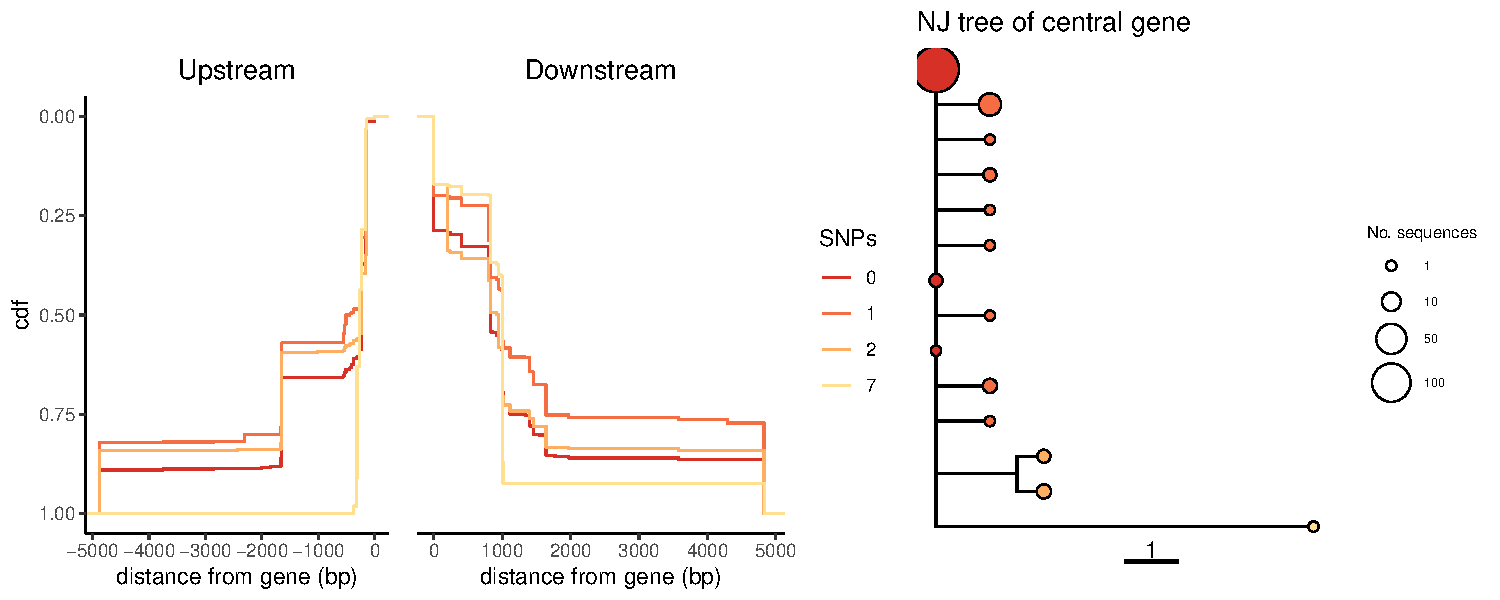
\includegraphics[width=\linewidth]{figs/CMY-2-mmseqs2-polish.all_u5000_d5000_pangraph.json.output_dists.csv.flanking-plot-output-focal-gene-seq.pdf}
    \caption{Structural diversity around CMY-2.}
    \label{fig:CMY-2}
\end{figure}


\subsection{Upstream diversity exceeds downstream diversity}

% Plot of Escherichia plasmids showing the following genes: CMY-2, CTX-M-15, CTX-M-65, KPC-2, NDM-1, OXA-1, TEM-1
% 

\section{Conclusion}

Limitations: transposition events can cause small-scale (2-bp) insertions. These are well below the size limit of pangraph used (default: 100bp). This means that more fine-grained analysis is certainly possible. Analysing this way gives us a coarse-grained / fuzzy picture. 

\section{Acknowledgements}

\noindent LPS is a Sir Henry Wellcome Postdoctoral Fellow funded by Wellcome (Grant 220422/Z/20/Z). RAN is funded by the University of Basel and the NSF. 



\section{Data availability}

\noindent Code and data (NCBI accessions) to reproduce analyses are available at \url{https://github.com/liampshaw/beta-lactamases}. 

\bibliography{cite}{}

\end{document}